\documentclass[a4paper,12pt]{article} %style de document
\usepackage[utf8]{inputenc} %encodage des caractères
\usepackage[french]{babel} %paquet de langue français
\usepackage[T1]{fontenc} %encodage de la police
\usepackage[top=2cm,bottom=2cm,left=2cm,right=2cm]{geometry} %marges
\usepackage{graphicx} %affichage des images
\usepackage{amssymb}
\usepackage{url}
\usepackage{verbatim}
\usepackage{amsmath}
\usepackage{color}
\usepackage{tikz}
\usepackage{hyperref}
\usepackage{float}
\usepackage{listings}
\lstset{
    language=bash, %% Troque para PHP, C, Java, etc... bash é o padrão
    basicstyle=\ttfamily\small,
    numberstyle=\footnotesize,
    numbers=left,
    backgroundcolor=\color{gray!5},
    frame=single,
    tabsize=2,
    rulecolor=\color{black!30},
    escapeinside={\%*}{*)},
    breaklines=true,
    breakatwhitespace=true,
    framextopmargin=2pt,
    framexbottommargin=2pt,
    inputencoding=utf8,
    extendedchars=true,
    literate={á}{{\'a}}1 {ã}{{\~a}}1 {é}{{\'e}}1,
}
\hypersetup{
	hidelinks,
    colorlinks,
    citecolor=black,
    filecolor=black,
    linkcolor=black,
    urlcolor=black
}

\begin{document} %début du document

%----------------------------------
%page de garde
%----------------------------------

\begin{titlepage}


\includegraphics[scale=0.3]{images/unicaen.png}

\vspace{7cm}

\begin{center}

\begin{Huge}
Rapport de Projet Tutoré\\
\end{Huge}
\vspace{1cm}
\begin{huge}
Expériences sur les nombres premiers\\
\end{huge}
\vspace{2cm}
\begin{large}
Beauchamp Aymeric 21301016\\
Chagneux Dimitri 21606807\\
Mori Baptiste 21602052\\
Leblond Valentin 21609038\\
\vspace{1cm}
L3-Informatique
\end{large}

\end{center}
\end{titlepage}


%------------------------------
%sommaire
%------------------------------

\newpage

\tableofcontents

\newpage

%------------------------------
%contenu
%------------------------------


\section*{Présentation du sujet}
\addcontentsline{toc}{section}{Présentation du sujet}

Les nombres premiers sont un des objets mathématiques les plus étudiés, de par l'ancienneté de leur découverte et leurs nombreuses propriétés.\\
En informatique, ils ont plusieurs applications : fonctions de hash, générateurs aléatoires, cryptographie asymétrique...
Dans ce projet, nous avons choisi de nous pencher sur certains aspects de ces nombres.\\

Nous avons travaillé sur plusieurs axes: les tests de primalité, les nombres de Mersenne, la spirale d'Ulam et la suite de Syracuse. Nous n'avons donc pas uniquement travaillé sur les nombres premiers.

\section{Détection des nombres premiers}
\subsection{Crible d'Eratosthène}
Le crible d’Ératosthène est un moyen très simple de de trouver les nombres premiers en partant de 2. Mais il y a plusieurs inconvénients quant à l'utilisation de cet algorithme.

\subsubsection{Fonctionnement}

Le crible d’Ératosthène se décompose en deux phases :
\begin{itemize}
\item Une première phase d'initialisation qui consiste à remplir une liste commençant à 2 et finissant au nombre jusqu'au quel nous voulons chercher des nombres premiers.\\
\item La seconde phase consiste à passer la liste au crible pour isoler les nombres premiers : pour cela on parcourt la liste de nombres ; pour chaque nombre on reparcourt cette liste et on supprime tous ses multiples.\\
\end{itemize}
Une amélioration simple consiste à mettre 2 dans la liste lors de l'initialisation puis à entrer tous les nombres allant de 3 à la limite que l'on veut avec un pas de 2.


\subsubsection{Benchmark}

Le graphique suivant montre le temps que met l'algorithme pour calculer de 2 jusqu'à la limite.\\
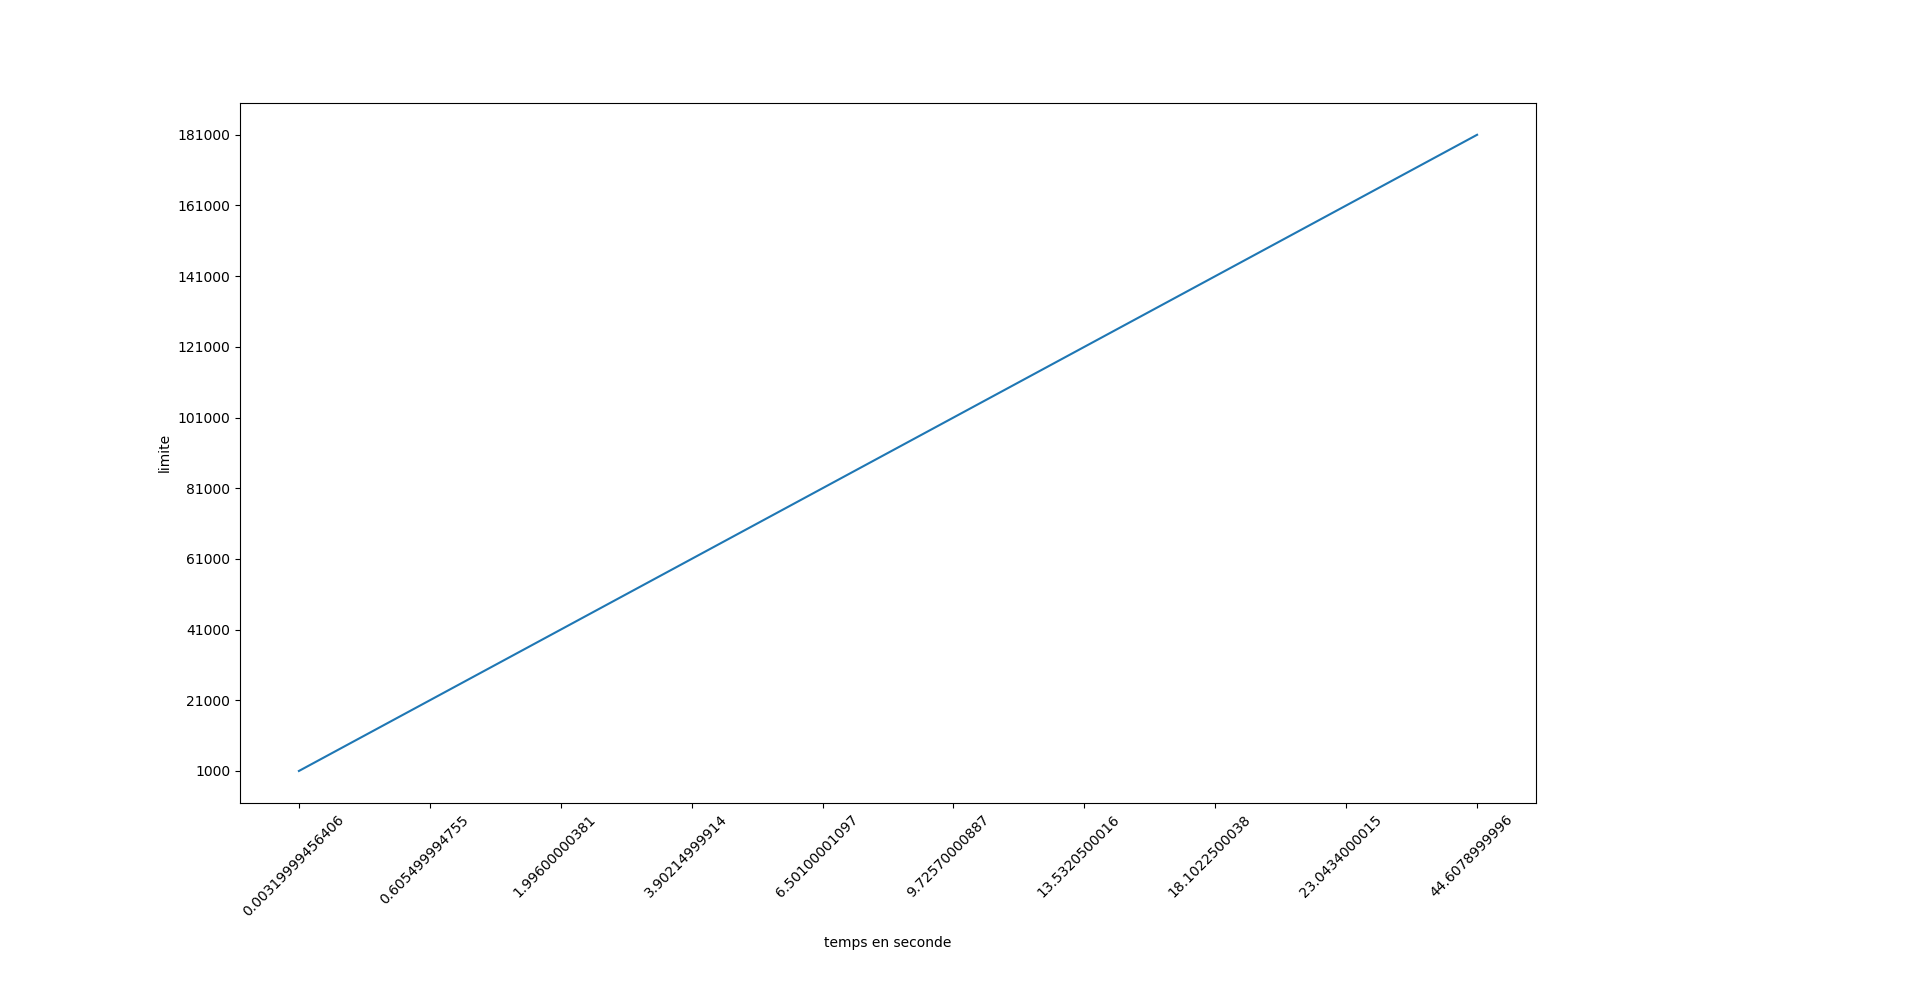
\includegraphics[scale=0.4]{images/erathostene1.png}
Comme on peut le voir, que alors que la limite augmente de façon linéaire ( de 20 000 en 20 000 ) alors que le temps lui augmente en $n^2$.\\


\subsection{Petit théorème de Fermat}
Le petit théorème de Fermat permet assez simplement de déterminer si un nombre est premier ou non. Cependant le processus peut prendre un certain temps.\\

\subsubsection{Fonctionnement}

Notre implémentation du petit théorème de Fermat fonctionne avec de l'aléatoire. On tire cinq fois un nombre \textit{a} aléatoire, allant de 1 à $p-1$ où \textit{p} est le nombre dont on souhaite déterminer la primalité. Le nombre de tirages a été choisi arbitrairement, cependant plus celui-ci est élevé moins le théorème se trompe.\\
Une fois le nombre \textit{a} tiré, on effectue un test avec un modulo. Le test est le suivant:\\
\begin{center}
$a^{p-1} \equiv 1$ (mod p)
\end{center}
Si ce test est faux, le nombre n'est pas premier donc on arrête le programme. Si il est juste, on continue avec de nouvelles valeurs pour \textit{a}. Si aucun des tests ne renvoie faux, le nombre a de très grandes chances d'être premier.

\newpage
\subsubsection{Benchmark}

Les captures suivantes montrent le temps de calcul de notre test de primalité basé sur le petit théorème de Fermat pour les nombres suivants: 733, 8 923, 109 547, 3 000 000 et 9 999 991.\\

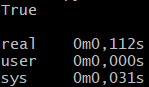
\includegraphics[scale=1]{images/fermat1.png}
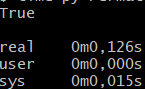
\includegraphics[scale=1]{images/fermat2.png}
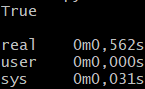
\includegraphics[scale=1]{images/fermat3.png}
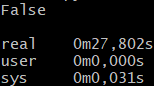
\includegraphics[scale=1]{images/fermat4.png}
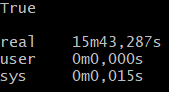
\includegraphics[scale=1]{images/fermat5.png}
\\
Comme on peut le constater, le temps de calcul augmente très rapidement et devient vite trop important avec 15 minutes pour 9 999 991. Il est rapidement trop long de tester la primalité d'un nombre. C'est pourquoi nous avons mis en place une fonction d'exponentiation modulaire.

\subsection{Exponentiation modulaire}
\subsubsection{Fonctionnement}
L'exponentiation modulaire est un moyen très efficace d'améliorer la vitesse de calcul d'un exposant.\\

Son fonctionnement est simple: on souhaite calculer un nombre \textit{a} à la puissance \textit{e} modulo un nombre \textit{m}. On commence par tester si \textit{e} modulo 2 est égal à 1. Si c'est le cas, on divise \textit{e} par 2, sinon on divise $e-1$ par 2. On continue ainsi jusqu'à ce que \textit{e} soit égal à 0.
Ainsi, à chaque itération l'exposant est divisé par 2.\\

Notre implémentation utilise les opérateurs binaires de Python. Dans notre fonction d'exponentiation modulaire, on utilise le code \textit{$e\&1$} pour tester si \textit{e} modulo 2 vaut 1. Pour diviser par 2, on effectue un décalage d'un bit à droite avec l'opérateur $\gg$.
Le nombre \textit{a} passé en argument est un nombre quelconque compris entre 1 et un nombre $p-1$ où \textit{p} est le nombre dont on souhaite déterminer la primalité. \textit{e} devient donc $p-1$ et \textit{m} devient \textit{p}. A chaque itération de boucle (sur l'exposant $p-1$), on donne à \textit{a} la valeur $a^2 $ modulo p.
\subsubsection{Benchmark}

Les captures suivantes montrent le temps de calcul du test de primalité utilisant l'exponentiation modulaire pour les mêmes nombres que ceux utilisés pour les benchmark du petit théorème de Fermat, à savoir: 733, 109 547, 3 000 000 et 9 999 991.\\

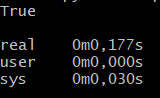
\includegraphics[scale=1]{images/expo1.png}
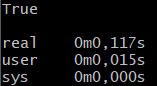
\includegraphics[scale=1]{images/expo2.png}
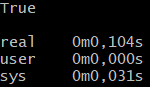
\includegraphics[scale=1]{images/expo3.png}
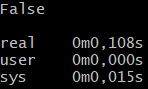
\includegraphics[scale=1]{images/expo4.png}
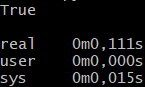
\includegraphics[scale=1]{images/expo5.png}

Cette fois-ci, contrairement au petit théorème de Fermat, le temps de calcul n'augmente pas. On peut donc déterminer si un nombre est premier très rapidement.\\
Ainsi le temps de calcul du test de primalité d'un très grand nombre comme 837 561 084 est de :

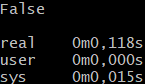
\includegraphics[scale=1]{images/expo6.png}

\subsubsection{Utilisation dans le petit théorème de Fermat}
Afin de rendre le calcul de primalité du petit théorème de Fermat plus performant, on peut remplacer le test $a^{p-1} \equiv 1$ (mod p) par un appel à la fonction d'exponentiation modulaire. L'exponentiation modulaire retourne combien de fois on a divisé l'exposant moins un par 2. Si un nombre est premier, on a effectué une et une seule division. Donc si la fonction retourne un nombre supérieur à 1, le nombre n'est pas premier.\\
Ainsi, comme on peut le voir en comparant les benchmarks, l'exponentiation modulaire permet de définir si un nombre est premier en un temps très petit et quel que soit ce nombre.

\subsection{Comparaison entre crible d'Eratosthène et petit théorème de Fermat}
\begin{itemize}
\item L'un des inconvénients du crible d’Ératosthène est que lors de l'initialisation, on stocke les nombres de 1 à une limite n, définie arbitrairement, dans une liste, ce qui peut prendre beaucoup de place en mémoire si la limite est élevée. On ne peut donc pas traiter une grande liste si on a pas suffisamment de place en mémoire.\\

\item Pour commencer à traiter une liste, il faut forcément commencer à 2 car on retire les multiples de chaque nombre traité de la liste. Donc on ne peut pas commencer à un nombre strictement supérieur à 2 si on ne veut pas oublier les multiples de 2.\\
Cela implique que si on veut arrêter le programme, il faut sauvegarder l'état courant, ce qui prend un peu plus de place en mémoire.\\

\item Contrairement au petit théorème de Fermat, qui lui teste les nombres de façon indépendante, le crible d’Ératosthène n'est pas parallélisable car on enlève les multiples du nombre que l'on traite dans la même liste, deux threads ou processus ne peuvent donc pas accéder à cette liste en simultané. Donc on traite moins de nombres à la fois.\\
\end{itemize}

Sur les screens suivants, on peut voir la différence de temps que mettent le crible d’Ératosthène (premier screen) et le petit théorème de Fermat (second screen) pour générer une liste de nombres premiers allant de 3 à 1 000 000.\\

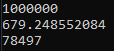
\includegraphics[scale=1]{images/eratosthene_1000000.png}
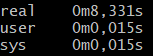
\includegraphics[scale=1]{images/comp_fermat.png}\\
Sur la première image, réalisé à partir du crible d'ératosthène, pour chercher les nombres premiers entre 2 à 1 000 000 on met 679s ce qui équivaut à 11 min et on a trouvé 78497 nombres premiers.\\


\subsection{Génération de polynôme}
\subsubsection{Idée de départ}
Dans le but d'améliorer la recherche de nombres premiers, nous avons travaillé sur la génération de polynôme de degré 2 dont les valeurs successives sont des nombres premiers.\\
Lors de quelque recherche personnelle je suis arrivé sur l'interpolation Lagrangienne, ce qui nous a conduit utilisé cette méthode avec 3 nombres premier consécutifs pour produire un polynôme de degré 2 qui génére ces 3 nombres.\\ Ce qui nous permet d'avoir des polynôme de degré 2 qui générent au minimum 3 nombres premier de maniére consécutive pour pouvoir itérer dessus.\\
\subsubsection{Fonctionnement}
L'algorithme de génération de polynôme de degré 2 est très simple, il se décompose en 2 parties. Une première partie est l'interpolation Lagrangienne des 3 nombres premiers et la seconde l'itération de ce polynôme.\\

\lstinputlisting[language=Python]{../python/poly_pseudo_algo.py}



\subsubsection{Résultat obtenue}
Lors de plusieurs test nous avons peu trouver un polynôme permettant de générer 40 nombres premiers consécutif, ce polynôme est celui que Euler à découvert en 1772.\\ Il est formé par les coefficients $n^2$+n+41, qui pour n allant de 0 à 39 génère 40 polynômes consécutif. Nous avons retrouvé ce polynôme grâce à l'interlation des nombres premiers 41 43 et 47 pour x prennant les valeurs respectives 0 1 et 2.\\ Sinon à part ce polynôme nous n'avons eu aucun résultats significatif.


\subsection{Conclusion}
Nous avons cherché un moyen de tester la primalité d'un nombre sans générer toute une liste. Puis lorsque nous avons vu que le petit théorème de Fermat permettait de calculer plus rapidement une liste de nombres premiers que le crible d’Ératosthène, nous l'avons utilisé pour générer une liste.\\

Par la suite nous avons grandement amélioré le temps de calcul du petit théorème de Fermat à l'aide de l'exponentiation modulaire.\\

Grâce à ce procédé, nous avons pu générer environ un milliard quatre-cent cinquante millions de nombres premiers en à peu près trente heures, contrairement au crible d’Ératosthène qui nous a permis de trouver seulement trente-cinq mille nombres premiers en soixante heures.

\section{Nombres de Mersenne}
Les nombres de Mersenne sont les nombres qui s'expriment sous la forme :

\begin{center}
$M_{n} = 2^{n}-1, n\geq1$
\end{center}

A partir de cette séquence, on trouve la sous-suite des nombres premiers de Mersenne, composée comme son nom l'indique des nombres de Mersenne qui sont aussi premiers.\\
De par la simplicité de leur expression et la progression exponentielle de la suite, ces nombres battent régulièrement le record du plus grand nombre premier connu, le dernier en date étant $M_{82 589 933}$, un nombre constitué d'environ 25 millions de chiffres en base 10 découvert en décembre 2018.\\
Nous avons essayé de parcourir la suite des nombres de Mersenne pour trouver les termes premiers de deux façons différentes : via la recherche dans un fichier et via un test de primalité.

\subsection{Recherche des nombres premiers dans une liste}
Nous avons alors recherché les nombres premiers de Mersenne parmi une liste de 300 000 000 nombres premiers générée avec la méthode d'exponentiation modulaire décrite en première partie.
Avec cette méthode, le plus grand nombre de Mersenne trouvable est $M_{31}=2 147 483 647$.
Il a fallu environ deux heures pour trouver tous les nombres.

\subsection{Test de Lucas-Lehmer}
Le test de Lucas-Lehmer est un test de primalité spécifique aux nombres de Mersenne. Il fonctionne de la manière suivante :

Soit $s_{i}$ la suite définie par $s_{0}=4$ et $s_{i+1}=s_{i}^{2}-2$.
Pour $p>2$, $M_{p}$ est premier si et seulement si $s_{p-2} mod M_{p} = 0$.

Nous avons mesuré le temps nécessaire au test pour les nombres jusqu'à $M_{31}$ :
\begin{figure}[!h]
\begin{center}
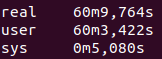
\includegraphics[scale=0.5]{images/benchmark_lucas.png}
\end{center}
\caption{Résultat du test de Lucas-Lehmer appliqué de $M_{3}$ à $M_{31}$}
\end{figure}

En outre, nous avons mesuré l'évolution du temps de calcul du test de primalité en fonction de l'indice dans la suite :
\begin{figure}[!h]
\begin{center}
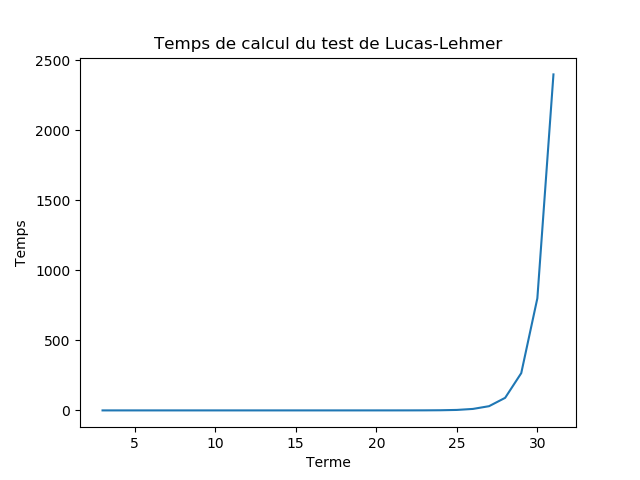
\includegraphics[scale=0.5]{images/evo_lucas.png}
\end{center}
\caption{Évolution du temps de calcul jusqu'à $M_{31}$}
\end{figure}

On observe que le temps de calcul augmente de façon exponentielle, ce qui était prévisible étant donné que le test est basé sur une suite définie par récurrence.\\

\subsection{Conclusion}
Si le test de Lucas-Lehmer est extrêmement rapide au début, il devient vite inefficace par rapport à une recherche dans une liste qui s'effectue en temps constant ; cependant l'utilisation d'un fichier crée un vrai problème de mémoire pour la recherche de grands nombres.


\section{Spirale d'Ulam}
La spirale d'Ulam consiste à avoir une grille de nombre remplie en forme de spirale et de marquer les nombres premiers.
\begin{figure}[!h]
\begin{center}
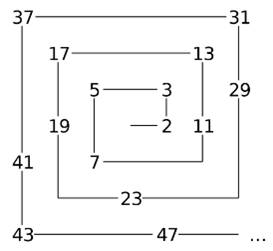
\includegraphics[scale=0.8]{images/spirale_explication.jpg}

\includegraphics[scale=0.3]{images/spirale_explication.PNG}
\end{center}
\caption{Spirale d'Ulam}
\end{figure}

\subsubsection{Réalisation}
Nous avons réalisé cette spirale en Java en utilisant la bibliothèque Swing. Pour la partie modèle, nous avons séparé le problème en deux classes : une qui modélise la grille (\textbf{Board}) et l'autre représentant un curseur (\textbf{Cursor}) en abstrait, qui pointera sur la case que la grille doit remplir et qui s'occupera de l'ordre de remplissage. Une implémentation de cette classe abstraite est \textbf{SpiralCursor} qui se déplacera en forme de spirale dans la grille (on pourrait bien évidemment envisager différents types de remplissage et il suffirait d'ajouter une nouvelle implémentation de curseur).\\ 
Un curseur s'utilise un peu de la même manière qu'un \textbf{Iterator} en Java, il prend en argument une grille et il se place à une certaine coordonnée et direction de départ. Il possède deux principales méthodes, \textbf{canMove} qui va tester si la case de la grille est déjà remplie à une distance d'une case dans la direction où le curseur est tourné, la seconde méthode est \textbf{next} qui fait avancer le curseur d'une case dans la direction vers laquelle il est tourné.\\

\begin{figure}[H]
\begin{center}
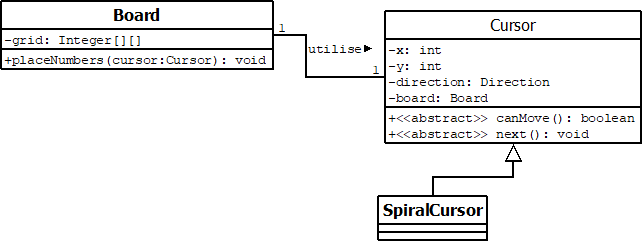
\includegraphics[scale=0.5]{images/dia_spirale.png}
\end{center}
\caption{Diagramme de classe pour la spirale d'Ulam}
\end{figure}

Ensuite, pour la partie graphique, nous avons simplement fait une fenêtre qui possède un \textbf{JPanel} sur lequel on va dessiner notre grille en ne remplissant que les cases qui possèdent un nombre premier en noir.

\begin{figure}[H]
\begin{center}
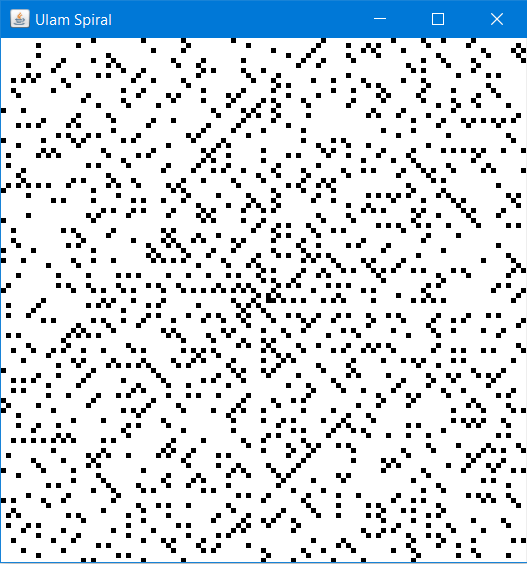
\includegraphics[scale=0.5]{images/swing_spirale.PNG}
\end{center}
\caption{Interface graphique de la spirale d'Ulam en Swing}
\end{figure}

Le test de primalité utilisé dans cette partie est simplement un parcours de 3 à $\sqrt{n} + 1$ avec un pas de deux. Il n'était pas nécessaire d'implémenter l'exponentiation modulaire car nous avons qu'une petite partie de nombre premiers donc la différence de temps aurait été faible.\\
\newpage
\lstinputlisting[language=Java, firstline=14, lastline=31]{../java/src/utilitaire/MyMath.java}

\subsubsection{Observations}
En prenant certaines valeurs de départ pour le remplissage de la spirale, on peut remarquer un alignement de nombres premiers, par exemple pour 41 on retrouve une ligne diagonale et pour 104 on peut apercevoir deux alignements parallèles en diagonale ainsi qu'une sorte de grand quadrillage.

\begin{figure}[H]
\begin{center}
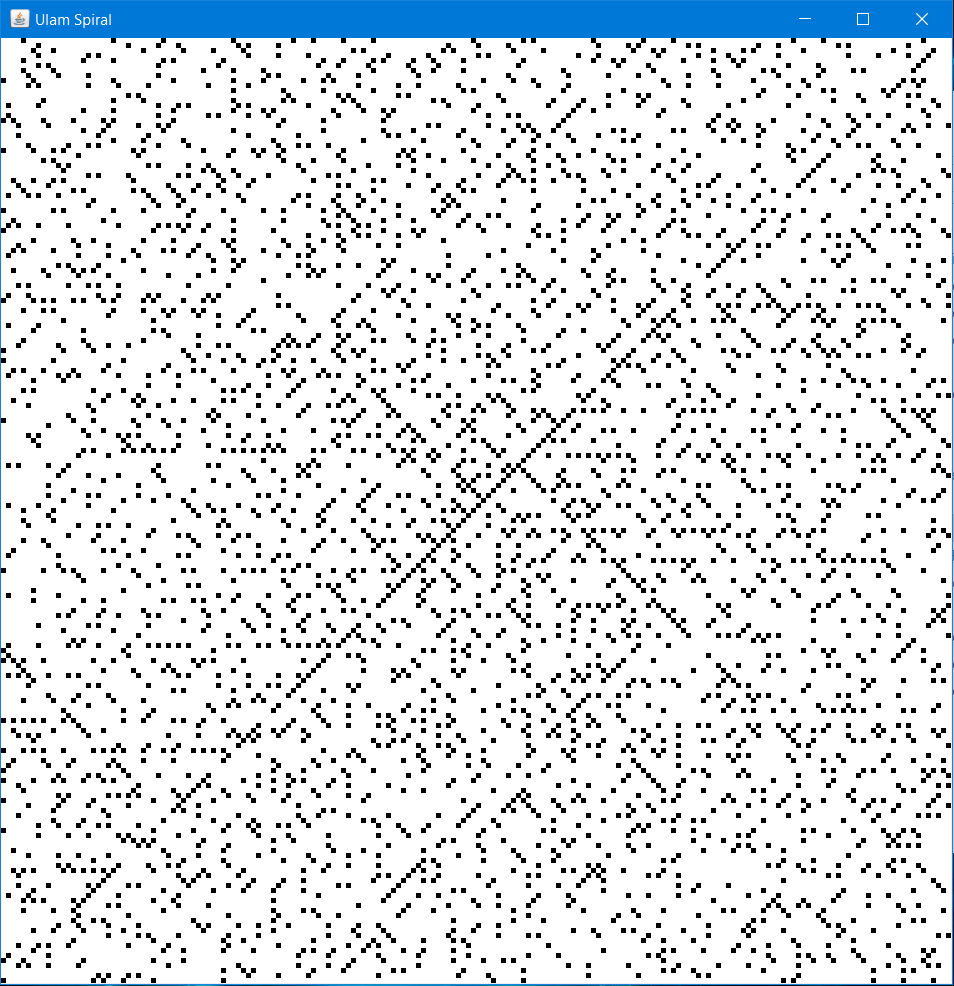
\includegraphics[scale=0.3]{images/spirale_41.PNG}
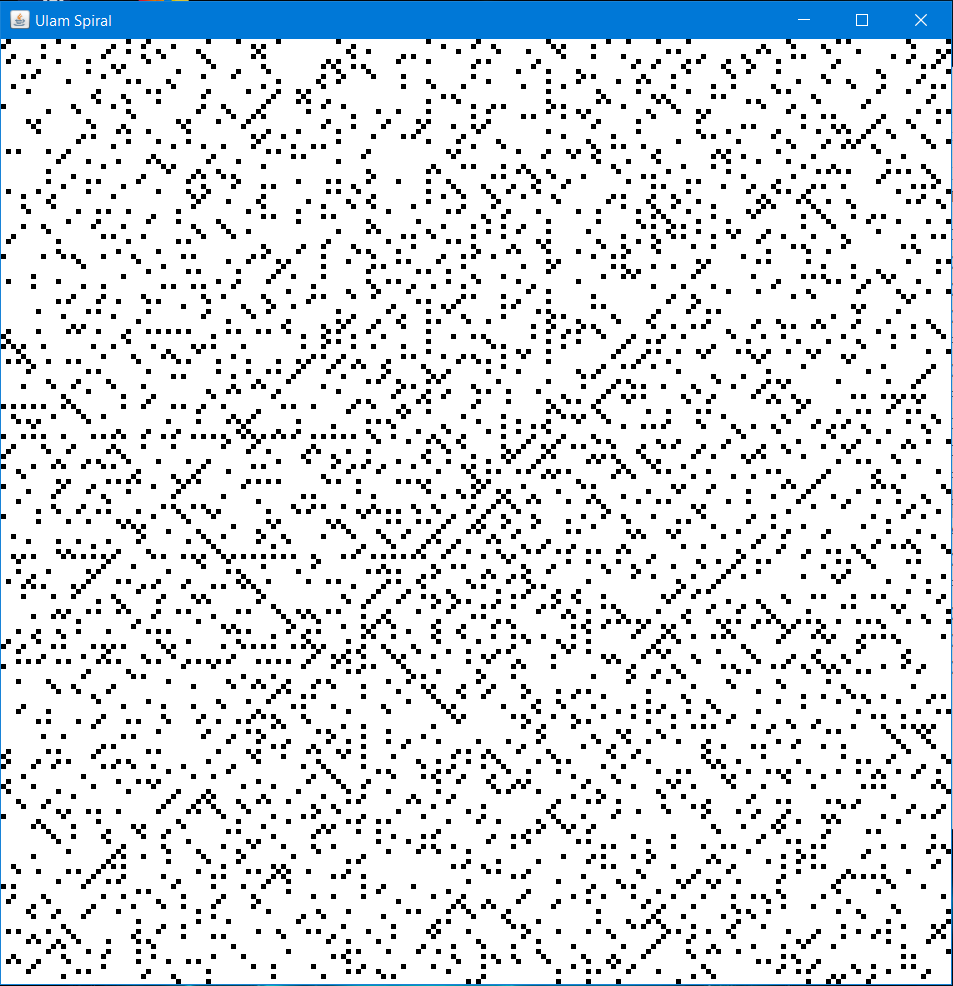
\includegraphics[scale=0.3]{images/spirale_104.PNG}
\end{center}
\caption{Spirale d'Ulam avec 41 (à gauche) et 104 (à droite) pris comme nombre de départ}
\end{figure}

Sachant qu'il y a une infinité de nombres premiers et que leur fréquence diminue logarithmiquement à mesure qu'on tend vers l'infini, c'est tout naturellement qu'on constate que les cases de nombres premiers sont plus condensées en commençant la spirale avec 1 qu'avec un plus grand nombre comme 1548468615.

\begin{figure}[H]
\begin{center}
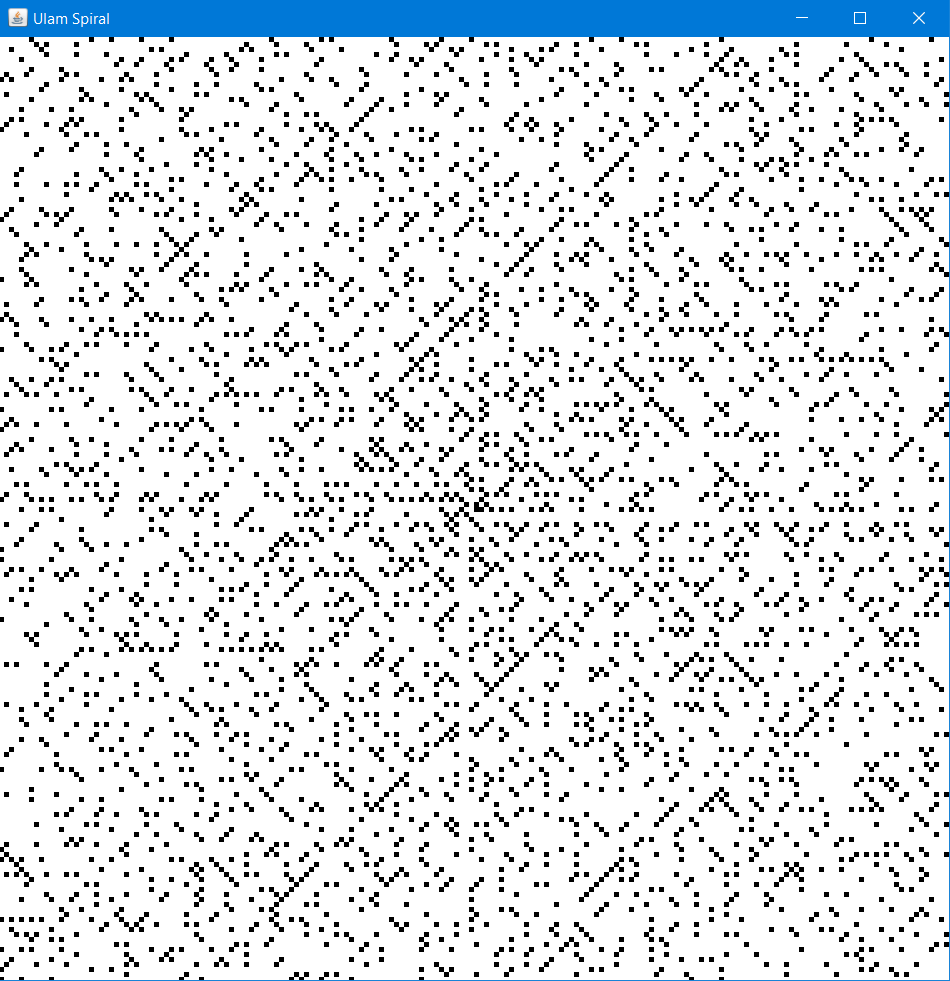
\includegraphics[scale=0.3]{images/spirale_1.PNG}
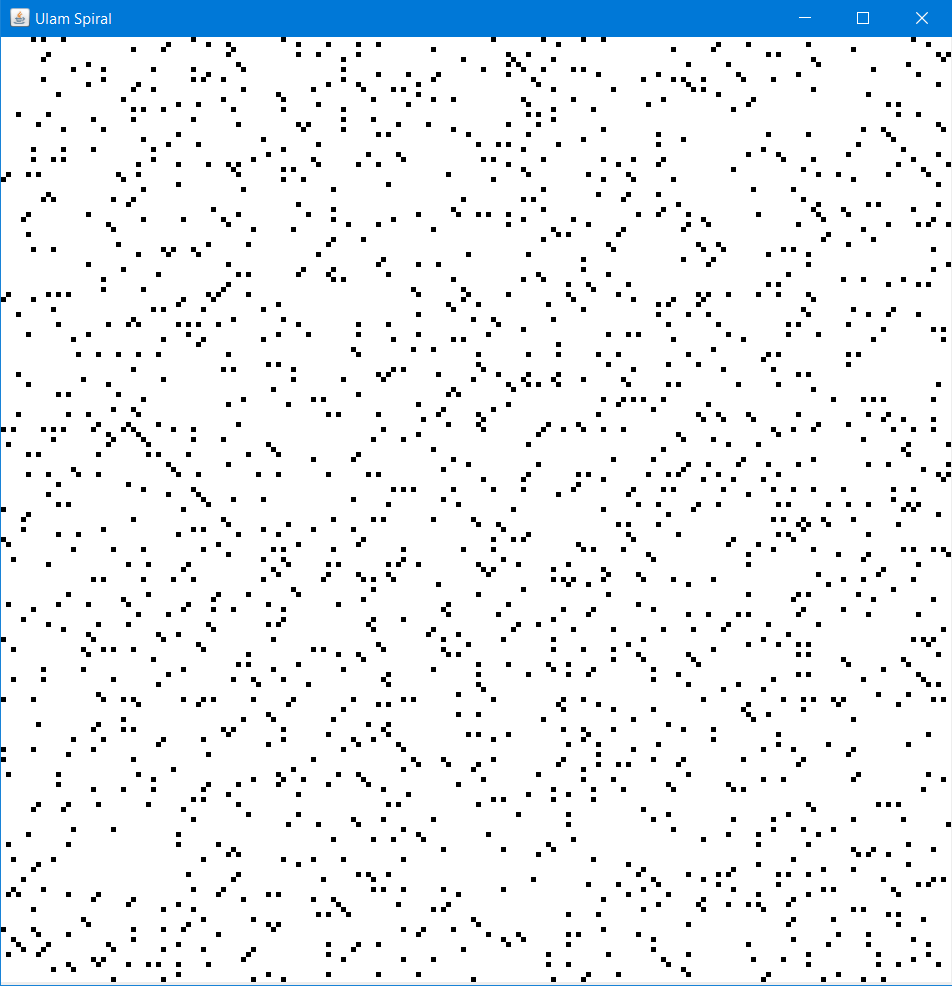
\includegraphics[scale=0.3]{images/spirale_grandNB.PNG}
\end{center}
\caption{Spirale d'Ulam avec 1 et 1548468615 pris comme nombre de départ}
\end{figure}




\section{Syracuse (3n+1)}
La suite de Syracuse s'exécute sur un nombre donné k qui consiste à diviser ce nombre par 2 si k est pair, ou le multiplier par 3 et lui ajouter 1 si celui-ci est impair ; on s'arrête quand on tombe sur 1. \\
On peut donc représenter cette suite de la manière suivante : \\ 

On a une suite $(U_n)$ avec $U_0 = k$ et 
$$
U_{n+1} = \left\{
    \begin{array}{ll}
        U_n/2 & \mbox{si } U_n \mbox{ pair} \\
        3*U_n + 1 & \mbox{si } U_n \mbox{ impair} \\
        1 \mbox{ fin} & \mbox{si } U_n = 1
    \end{array}
\right.
$$

Exemple sur 3 :
$$
U_0 = 3, U_1 = 10, U_2 = 5, U_3 = 16, U_4 = 8, U_5 = 4, U_6 = 2, U_7 = 1, fin.
$$

\subsubsection{Réalisation}
Pour la partie modèle, nous avons séparé en deux parties la suite de Syracuse. Dans la première, nous allons calculer la suite pour chaque nombre de 2 à la valeur que l'utilisateur donnera. Pendant le calcul de la suite sur un nombre on va compter le nombre d'itérations qu'il effectue dans la suite (en reprenant l'exemple sur 3, celui-ci effectue 7 itérations) et on stocke le nombre d'itérations dans une map (pour 3 on stocke la paire {3 => 7}). Si, pendant le calcul de la suite sur un nombre, on tombe sur un nombre dont le nombre d'itérations a déjà été calculé, on va additionner le nombre d'itérations que l'on a fait jusqu'ici avec le nombre d'itérations qu'on a stocké dans la map et cela correspondra au nombre d'itérations que le nombre effectue dans la suite de Syracuse. Dans la seconde partie, on va calculer la suite de Syracuse sur un nombre donné et on va stocker dans une liste chaque valeur obtenue (pour 3 la liste est [3, 10, 5, 16, 8, 4, 2, 1]).\\

Ensuite, pour la partie graphique, nous avons fait une première interface en Swing d'un graphique en barres correspondant à un nombre de 2 à n avec le nombre d'itérations dans la suite de Syracuse. On peut passer la souris sur le graphique et il indique en haut à gauche le nombre et son nombre d'itérations dans la suite (sur la Figure \ref{syra100}, on se trouve sur 97 qui fait 118 itérations dans la suite de Syracuse).

\begin{figure}[H]
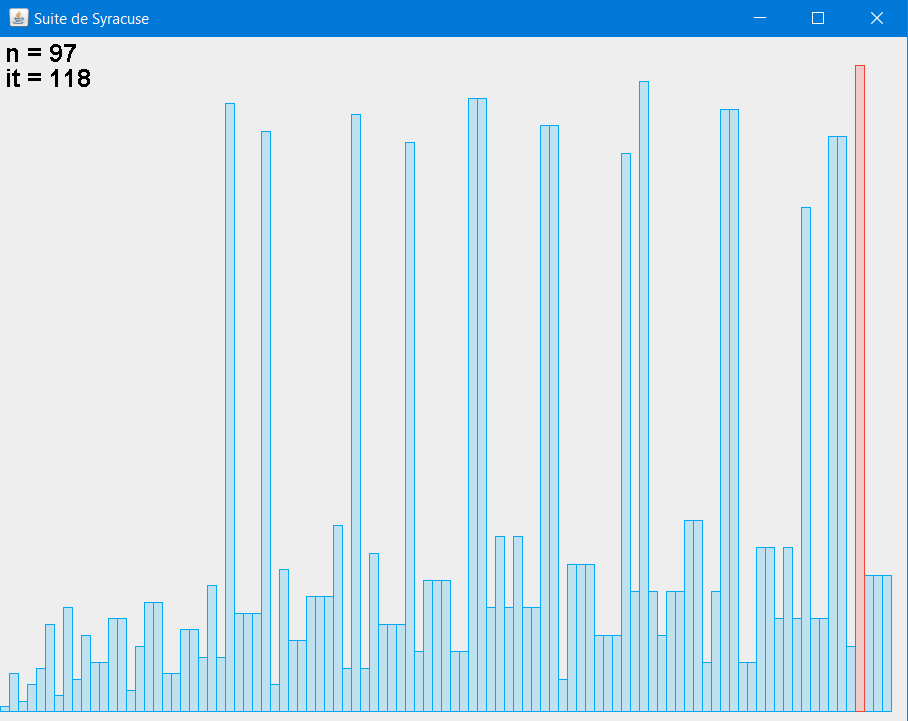
\includegraphics[scale=0.5]{images/syracuse_100.PNG}
\centering
\caption{Graphique de 2 à 100 en fonction de leur nombre d'itérations}
\label{syra100}
\end{figure}

La seconde interface porte sur les variations lors du calcul d'un nombre donné dans la suite de Syracuse. On peut passer la souris sur le graphique et il nous dit à quelle itération on est et la valeur actuelle (sur la Figure \ref{syra97}, on se trouve pendant la 84e itération avec une valeur de 9232).

\begin{figure}[H]
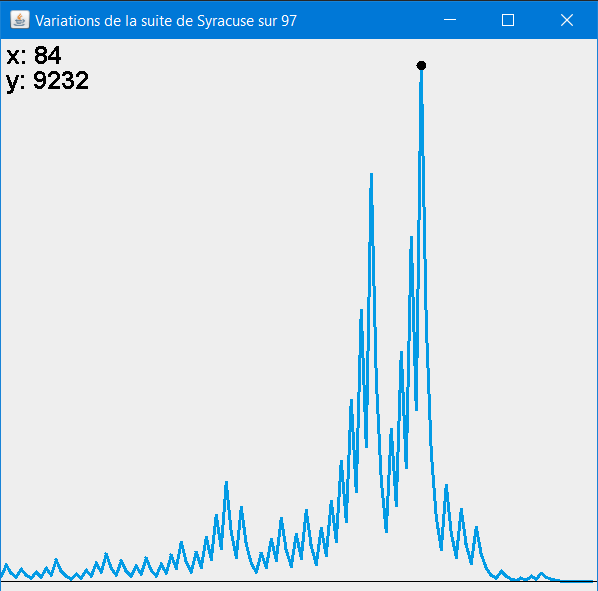
\includegraphics[scale=0.6]{images/syracuse_var_97.PNG}
\centering
\caption{Graphique sur de la variation dans la suite de Syracuse de 97}
\label{syra97}
\end{figure}

\subsubsection{Observations}

Pour la partie sur la comparaison du nombre d'itérations des différents nombres, on remarque que entre 2 et 100 (Figure \ref{syra100}), le nombre qui possède le plus grand nombre d'itérations est 97 avec 118 itérations. On remarque également qu'il y a plusieurs série de 2-3-5 nombres consécutifs qui ont le même nombre d'itérations, si on regarde entre 2 et 150, on a par exemple : 
\begin{itemize}
\item 12 et 13 avec 9 itérations
\item 28, 29 et 30 avec 18 itérations
\item 36, 37 et 38 avec 21 itérations
\item 44, 45 et 46 avec 16 itérations
\item 98, 99, 100, 101 et 102 avec 25 itérations
\item 130, 131, 132, 133 et 134 avec 28 itérations
\end{itemize}

Ensuite, sur les variations des nombres, on peur remarquer qu'on obtient des pics relativement importants sur des nombres qui ont un nombre important d'itérations. Pour 27, 31, 63, 73 et 97 (et probablement d'autres) on obtient la même valeur comme pic à 9232, comme si sur certains nombres on aurait une convergence vers une même fin qui commencerait à 9232.

\begin{figure}[H]
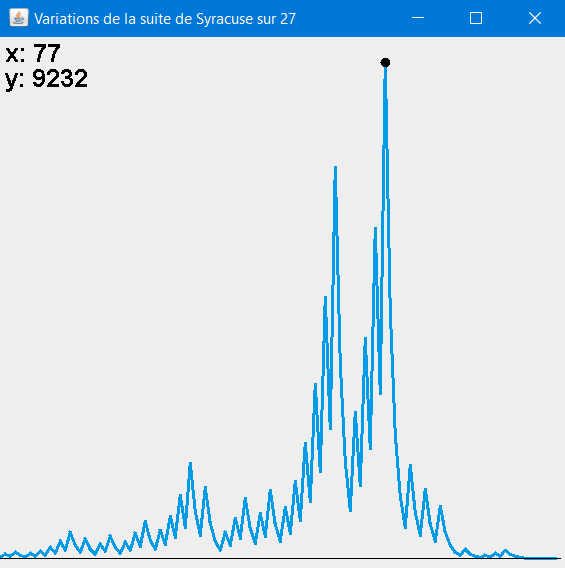
\includegraphics[scale=0.6]{images/syracuse_var_27.PNG}
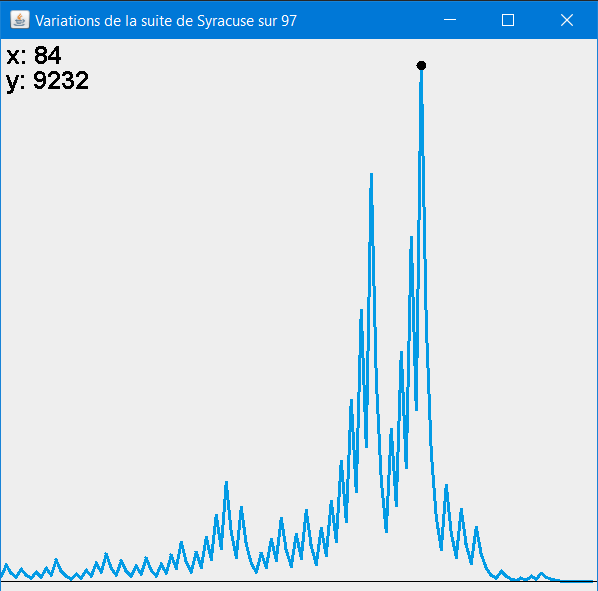
\includegraphics[scale=0.58]{images/syracuse_var_97.PNG}
\centering
\caption{Graphique sur de la variation dans la suite de Syracuse de 27 et 97}
\end{figure}

Les nombres qui ont la même fin de variations sont faciles à distinguer, ce sont tous les pics avec un écart plus important que la moyenne. Sur la figure \ref{pics}, toutes les valeurs étant au-dessus de la ligne rouge ont la même fin de variations commençant par 9232. Les nombres en dessous de la ligne rouge ont tous des variations tombantes comme celle de la Figure \ref{syra78} pour 68 et 78.

\begin{figure}[H]
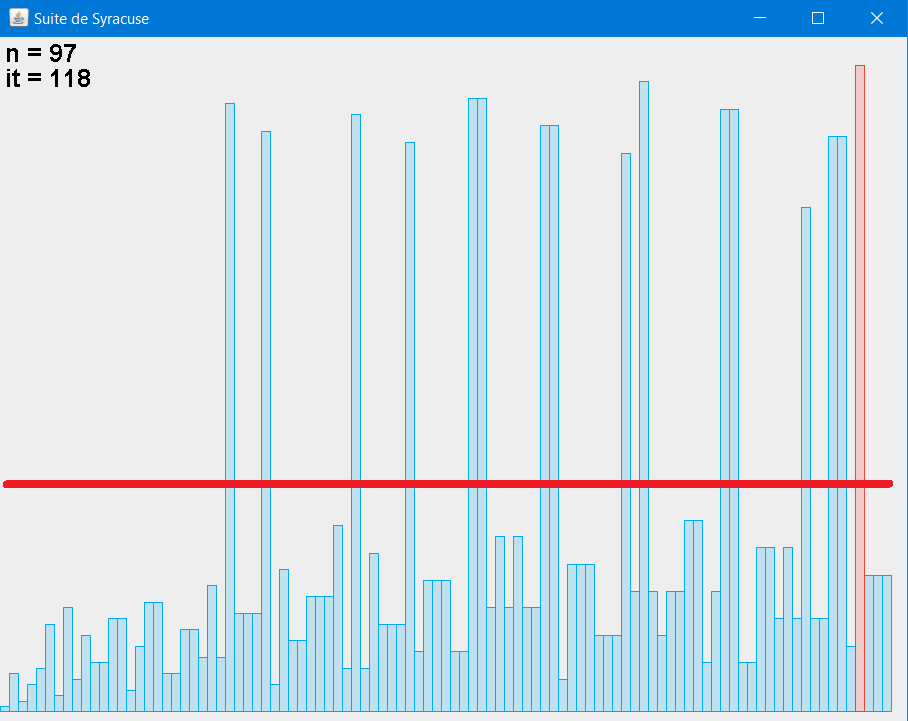
\includegraphics[scale=0.5]{images/syracuse_pics.PNG}
\centering
\caption{Graphique mettant en évidence les pics entre 2 et 100}
\label{pics}
\end{figure}

\begin{figure}[H]
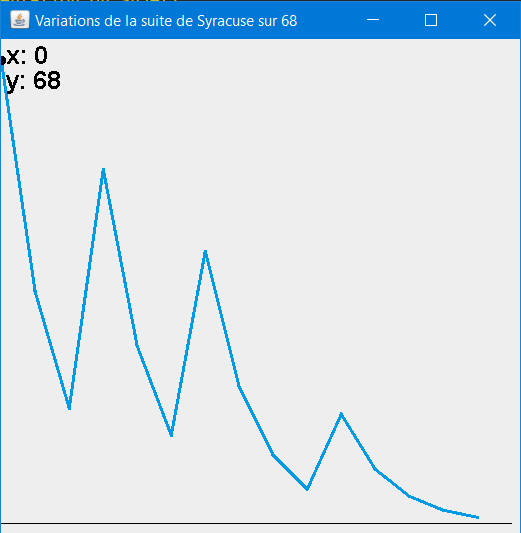
\includegraphics[scale=0.59]{images/syracuse_var_68.PNG}
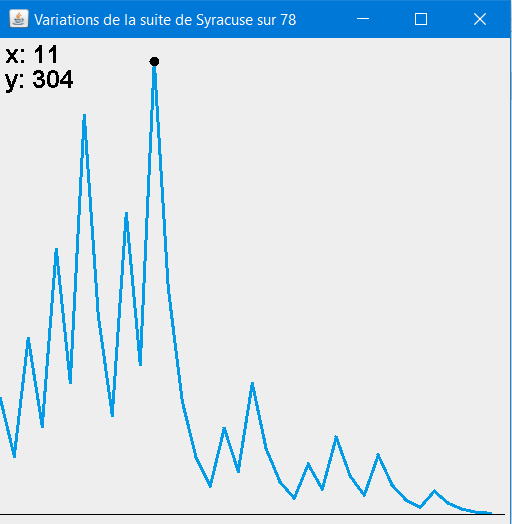
\includegraphics[scale=0.6]{images/syracuse_var_78.PNG}
\centering
\caption{Graphique sur la variation dans la suite de Syracuse de 68 et 78}
\label{syra78}
\end{figure}

\subsubsection{Test avec 5n+1}
Nous avons essayé d'utiliser la suite 5n+1 au lieu de 3n+1 ; seulement nous n'avons pas pu utiliser nos graphiques comme pour la suite 3n+1 car dans la suite il y a des valeurs pour lesquelles on se retrouve dans un cycle par exemple pour 5 on a un cycle 26, 13, 66, 33, 166, 83, 416, 208, 104, 52, 26, 13 ...\\
On obtient une suite qui a tendance a diverger si on prend par exemple 7. Si on prend 13 on retombe sur le cycle généré par 5 : 66, 33, 166, 83, 416, 208, 104, 52, 26, 13 ...






\section*{Conclusion}
\addcontentsline{toc}{section}{Conclusion}

Nous avons réussi remplir une grand nombre de nos objectifs qui consistaient à implémenter le crible d’Ératosthène, le petit théorème de Fermat, l'exponentiation modulaire, la spirale d'Ulam, la suite de Syracuse, les nombres de Mersenne et l'interpolation Lagrangienne pour générer des polynômes générateurs de nombres premiers.

Pour la partie polynôme générateur de nombres premiers, nous avons réussi à retrouvé le polynôme d'Euler mais le reste des résultats n'a pas été concluant.\\

Plusieurs améliorations sont possibles : pour le crible d’Ératosthène on aurait pu amélioré la liste qui stocke l'ensemble des nombres avec une liste chaînée afin de gagner de l'espace de stockage en modifiant directement cette liste.\\
Pour la recherche de nombres à partir d'un fichier expérimentée avec les nombres de Mersenne, on pourrait optimiser la recherche pour éviter de traiter toute la liste à chaque fois.\\

Ce sujet nous a permis d'étendre nos connaissances dans un domaine très vaste et toujours d'actualité, ainsi que d'utiliser nos compétences de plusieurs façons différentes. Le défi était de mélanger l'arithmétique et l'informatique afin de procéder à des calculs et faire de l'optimisation de fonctions.

\end{document}
